\chapter{Der Touchscreen}
Als Bildschirm von Shulker kann grundsätzlich jeder Touchscreen mit akzeptabler Größe verwendet werden.
Die Steuerung des Touchscreens wird von Shulker-Core mithilfe des crates \textbf{slint} (Version 0.2) übernommen.

\section{Funktionsweise von slint}
Um mit slint eine grafische Benutzeroberfläche bereitstellen zu können, wird empfohlen, eine slint-Datei zu erstellen.
In dieser Datei wird mittels der slint-Sprache eine Benutzeroberfläche beschrieben und programmiert. Diese Datei wird vom 
slint-Compiler in Binärcode umgewandelt. Da die .slint-Datei und der eigentliche Anwendungscode also getrennt sind, muss man sich
mittels Callbacks, Models und Eigenschaften verständigen.
\begin{figure}[H]
    \begin{center}
        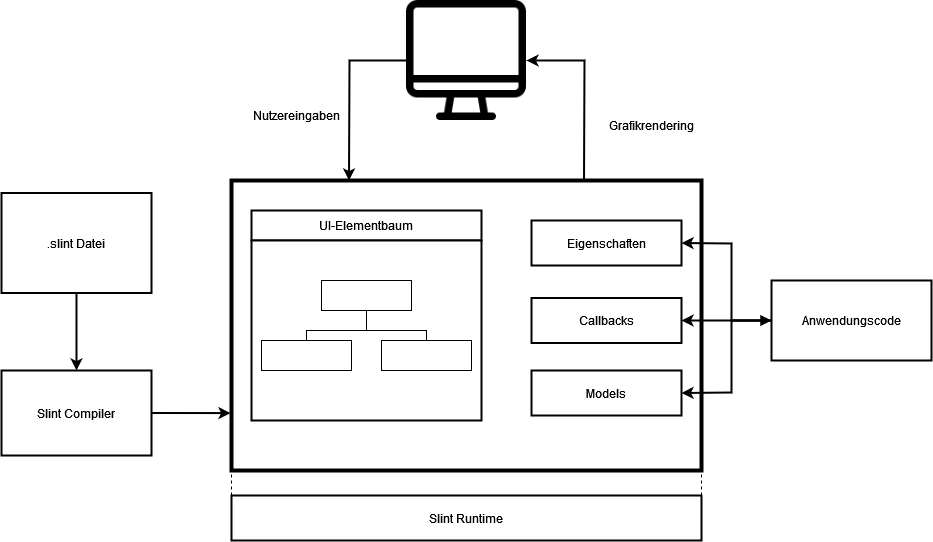
\includegraphics[width=0.9\textwidth]{images/core/slint_aufbau.png}
        \caption{Aufbau und Funktionsweise von slint \cite{slintfunktion}}
    \end{center}
\end{figure}

\section{Aufbau der grafischen Oberfläche}
Shulker-Core verwendet eine .slint-Datei, welche den Namen \textit{mainwindow.slint} trägt. Diese Datei befindet sich im Unterordner
namens \textit{ui} in der Git-Repository von Shulker. Das Design der Oberfläche konzentriert sich darauf, möglichst leicht
lesbar und stromsparend zu sein. Deshalb entschieden wir uns für die Farben Schwarz und Weiß.

Die grafische Oberfläche besteht aus drei Teilen:
\begin{itemize}
    \item Menü-Selektor
    \item Hauptansicht
    \item Unlocked-Ansicht
\end{itemize}

\subsection{Menü-Selektor}
Der Menü-Selektor ist grundsätzlich immer zu sehen. Die einzige Ausnahme bildet das Entsperrtsein des elektronischen
Schlosses. Der Menü-Selektor ermöglicht das Wechseln der Hauptansicht. Es gibt drei Wahlmöglichkeiten:
\begin{itemize}
    \item \textbf{Pin}: zur Eingabe von Ziffernpins
    \item \textbf{PW}: zur Eingabe von Passwörtern, also Pins mit Buchstaben
    \item \textbf{M}: zur Verbindung mit Shulker-Mobile
\end{itemize}

\subsection{Hauptansicht}
Die Hauptansicht nimmt den Großteil des Bildschirms in Anspruch. In ihr wird dem Nutzer das Eingeben von Pins und Passwörtern
ermöglicht. Ein QR-Code zur Verbindung mit Shulker-Mobile lässt sich auch anzeigen.

\begin{figure}[H]
    \begin{center}
        \includegraphics[width=0.99\textwidth]{images/core/ui_123.png}
        \caption{Core-UI mit den verschiedenen Hauptansichten: PIN, PW und M}
    \end{center}
\end{figure}

\subsection{Unlocked-Ansicht}
Die Unlocked-Ansicht zeigt dem Nutzer, dass das Schloss momentan offen ist. Sie nimmt den ganzen Bildschirm in Anspruch und weicht
als einzige Komponente vom standardmäßigen Farbschema ab; grelles Grün vermittelt ein klares Signal. Auf ihr ist auch ersichtlich,
wie lange das Schloss noch offen bleibt. Die Ansicht kann über mehrere Wege in den Vordergrund geschoben werden, grundsätzlich aber dann,
wenn an Shulker-Core ein Öffnen-Signal oder ein korrekter Pin gesendet wurde.

\section{Die Hardware}

\subsection{Vorzeigemodell}
Im Vorzeigemodell wird das offizielle \textit{Raspberry Pi Touch Display} verwendet. Der Bildschirm besitzt eine Auflösung von
800x480 Pixeln und hat eine diagonale Größe von sieben Zoll. Natürlich unterstützt er auch Berührungseingaben, um die Nutzbarkeit
von Shulker zu ermöglichen.

\subsection{Mögliche Displays}
Grundsätzlich kann Shulker-Core mit jedem Display, das mit dem Raspberry Pi kompatibel ist, arbeiten. Sollte ein besonders kleiner
Bildschirm gewählt werden, ist es äußerst wahrscheinlich, dass die standardmäßige Implementation des User-Interfaces nicht mehr
den Verhältnissen entspricht. Da das gesamte Projekt Open-Source und die Slint-Sprache nicht besonders komplex sind, kann
in solchen Fällen der Admin selbst eine eigenen Implementation der grafischen Benutzeroberfläche einbaun. Das ist natürlich auch von
Vorteil, wenn man zusätzliche Funktionen hinzufügen will.